\chapterauthor{Ricardo H. R. Lima}{Federal University of Paran\'a}
\chapterauthor{Vidal Fontoura}{Federal University of Paran\'a}
\chapterauthor{Aurora Pozo}{Federal University of Paran\'a}
\chapterauthor{Roberto Santana}{University of the Basque Country}


%TODO make contribuition clear

\chapter{Multi objective approach to the Protein Structure Prediction Problem}


\section{Introduction} \label{sec:intro}


Proteins play a fundamental task in nature, participating in many of the most important functions of living cells. These structures guarantee the correct functioning of a large number of biological entities in nature. The protein structures are the result of the so-called protein folding process in which the initially unfolded chain of amino-acids is transformed into its final structure. Under suitable conditions, this structure is uniquely determined by its sequence \cite{santana2004protein}. The prediction of protein structures has a wide range of important biotechnological and medical applications, e.g, design of new proteins and folds \cite{rothlisberger2008kemp, wang2012structural}, structure based drug design \cite{qian2004improvement, krieger2009improving} and obtaining experimental structures from incomplete nuclear magnetic resonance data \cite{shen2009novo, raman2009accurate}.


%Given its complexity, using a representation close to the real would be impossible for current computers to process the information in a reasonable time.
The determination of the final structure of a protein is a complex and challenging task even for modern super computers. This happens because  it would require a huge exponential time to sample all possible configurations that a given protein sequence could adopt. Although very detailed representation of proteins exists and can be used to model the proteins folding, these representations are computationally very costly. This is why many authors as in \cite{custodio2004investigation, hsu2003growth, krasnogor2002multimeme, lin2011protein, unger1993genetic} among others, use simplified models to represent the protein structures. A well known model for this purpose is the \textit{Hydrophobic-Hydrophilic} model (HP model), created by Lau and Dill \cite{lau1989lattice}. Considering just two types of residues H and P in a regular lattice, makes easier to represent a protein and work with it to simulate the folding process.


Although the HP model allows a great flexibility for explaining the space of possible folds, the manipulation of a protein structure represented in the HP model requires some attention in order to respect the given problem and avoid unfeasible conformations. Another issue is the difficulty in finding good measures to verify the quality of the simplified protein conformation represented by the solution. The most common measure used for the HP model is to calculate the conformation's energy based on the number of hydrophobic contacts that exist in the fold. The question then arises of how to search for the protein configurations that optimize the energy.

%But sometimes just the energy measure is not enough, being necessary the use of a second objective to avoid treating different solutions with the same energy value as being the same, for example.
Different heuristic approaches have been developed to decrease the computational complexity related to the protein structure determination process. Mono and Multi-objective methods have been used \cite{custodio2004investigation, hsu2003growth, krasnogor2002multimeme, lin2011protein, unger1993genetic,santana2008protein,gabriel2012algoritmos}, to find the simplified protein fold that are optimal given one ore more criteria.

 These approaches make use of optimization techniques like Genetic Algorithms \cite{unger1993genetic}, Ant Colony Optimization \cite{shmygelska2002ant, shmygelska2003improved}, Memetic Genetic Algorithms \cite{krasnogor2002multimeme}, Estimation of Distribution Algorithms \cite{santana2008protein}, and Multi-Objective Evolutionary Algorithms \cite{gabriel2012algoritmos}. However, with few exceptions most of previous approaches consider single-objective problem formulations and this motivated the presented chapter. 
 
% there is lack of works that explore multi-objective approaches and this motivated the presented chapter. 

 
This work proposes the application and comparison of a multi-objective approach to the Protein Folding Problem, considering two objectives. Using a multi-objective approach other characteristics of the protein, and not only its energy can be investigated. The main objective is to minimize the energy calculated from the HP model, and the second objective consists of minimizing the euclidean distance between amino acids of a protein. The introduction of the second objective was inspired by the work of Gabriel et al. [12], in which it is mentioned that the evaluation of a structure represented by the HP model considers only the number of hydrophobic contacts, what does not enable the optimization algorithms to distinguish between structures with the same number of hydrophobic contacts. Using a multi-objective approach other characteristics of the protein, and not only its energy can be investigated. In particular, in this chapter we investigate the distance because more compact structures tend to have more hydrophobic contacts: as lower the euclidean distance between the amino acids is, more compact the whole conformation will be.

% Another motivation for using the second objective is that more compact structures tend to have more hydrophobic contacts: as lower the euclidean distance between the amino acids, more compact the whole conformation will be. 

  
Two pareto based multi-objective evolutionary algorithms (MOEAs), NSGAII \cite{deb2002fast} and IBEA \cite{zitzler2004indicator}, were used, because they are well known MOEAs \cite{CoelloCoello2007} that use effective mechanisms to guarantee a good diversity of the Pareto front approximation, e.g, crowding distance mechanism and sophisticated measures to evaluate the quality of the solutions from a multi-objective point of view. Also their success when applied on the domain of other problems motivated their use in the context of this chapter.


Two versions of each algorithm were evaluated: one with the algorithms as they were originally specified and other with modifications in the initialization and mating process. A backtrack strategy is used to generate the initial population to avoid the generation of many invalid solutions. Therefore, the MOEAs will spend less time processing invalid solutions. The mating process is an important step in evolutionary algorithms. Since, it is the responsible to properly explore the search space applying the crossover and mutation operators. In multi-modal search spaces, with a lot of local optima, it makes sense to have sufficient operators that searches either for higher quality and diversified solutions, depending on the region of the search space that a given EA might be stucked in. Therefore, providing evolutionary algorithms with both kind of operators it have a big probability to better explore the search space in order to avoid local optima spots and also to exploit valleys of the search space. The mentioned modifications changes were introduced because the initial experiments showed that the standard MOEAs were not able to achieve satisfactory results. Another motivation for this chapter was the use of Pareto based algorithms in order to explore the performance of this type of algorithms when applied to the PSP problem. 


%TODO: Improve the motivation (multimodal many local optima, satisfy the constraints)

%TODO: Try to improve the motivation of the operators and backtrack strategy later in the conclusions or in the proposed method 
 

%We then validate the combination of enhancement techniques conceived for the HP problem with the original NSGAII and IBEA variants and  show that in terms of the HV our proposal produces better results. Furthermore, we show that in terms of the energy of the protein configurations found, our method is competitive with previous single-objective approaches.
   


 
% The evolutionary algorithms NSGAII and IBEA were used, considering some different strategies for the operators and initialization. The results of the experiments are compared with other well-known techniques and discussed to evaluate its performance. 
 
 
 %This leave a window of opportunities speaking about well-known pareto based algorithms like NSGAII \cite{zitzler1998multiobjective} and IBEA \cite{zitzler2004indicator} which have been extensively applied in other real-world problems.
 
 
 %The main difference between the mentioned methods \cite{custodio2004investigation, hsu2003growth, krasnogor2002multimeme, lin2011protein, unger1993genetic}, is that NSGAII and IBEA are multi-objective algorithms, and different from a GA, have more sophisticated mechanisms to evolve the population and try to improve the solutions. 

%TODO: IMPROVE THIS PART

The remainder of this chapter is organized as follows, we briefly introduce the main aspects of the Protein Folding Problem and a review of the related works is also presented. Section \ref{sec:optimization} reviews the Multi-Objective optimization context and the NSGAII and IBEA algorithms are presented. Thereafter, in Section \ref{sec:proposedMethod} the proposed method is introduced. In Section \ref{sec:experiments}, the experimental benchmark and numerical results of the conducted experiments are presented. Finally, in Section \ref{sec:conclusion}, the conclusions of the research are given, and further work is discussed.

%This chapter is organized as follows. In Section \ref{sec:proteinfolding} are presented the main aspects of the Protein Folding Problem and important information for the research. Section \ref{sec:optimization} briefly presents the Multi-Objective optimization, showing the positive aspects that can help solving the PSP Problem. In Section \ref{sec:proposedMethod} is presented the description of the proposed method, and its relation to other methods presented in the previous works. The experiments are shown in Section \ref{sec:experiments} with information about the proposed method compared with other well-known works. Finally the conclusion and future works are discussed in Section \ref{sec:conclusion}.


\section{Protein Structure Prediction} \label{sec:proteinfolding}


Proteins are macromolecules made out of  twenty different amino acids, also referred to as residues. An amino acid has a peptide backbone and a distinctive side chain group. The peptide bond is defined by an amino group and a carboxyl group connected to an alpha carbon to which  a hydrogen and side chain group are attached.


Amino acids are combined to form sequences which are considered the primary structure of the peptides or proteins. The secondary structure is the locally ordered structure brought via hydrogen bounding mainly within the peptide backbone. The most common secondary structure elements in proteins are the alpha helix and the beta sheet. The tertiary structure is the global folding of a single polypeptide chain.


Under specific conditions, the protein sequence folds into a unique native 3-D structure. Each possible protein fold has an associated energy. The \emph{thermodynamic hypothesis} states that the native structure of a protein is the one for which the free energy achieves the global minimum. Based on this hypothesis, many methods \cite{custodio2004investigation, hsu2003growth, krasnogor2002multimeme, lin2011protein, unger1993genetic} that search for the protein native structure define an approximation of the protein energy and use optimization algorithms that look for the protein fold that minimizes this energy. These approaches mainly differ in the type of energy approximation employed and in the characteristics of the protein modeling.


\subsection{The HP Model} \label{sec:hpModel}


%Using a representation close to the real would be impossible for current computers to process the information in a reasonable time.
The protein structures are very complex. Detailed representation of protein exists and can be used to model the protein folding, these representations are computationally very costly. Having this in mind, Lau and Dill \cite{lau1989lattice} created a model called \textit{Hydrophobic-Hydrophilic} Model (HP Model), to represent the proteins using simplifications. The model can be used either to represent proteins in a 2D space or 3D space.


The HP model considers two types of residues:  hydrophobic (H) residues  and hydrophilic or polar (P) residues. A protein is considered a sequence of these two types of residues, which are located in regular lattice models forming self-avoided paths. Given a pair of residues, they are considered neighbors if they are adjacent  either in the chain (connected neighbors) or  in the lattice but not connected in the chain (topological neighbors).


\begin{figure}[htb!] \label{fig:PROTEXAM}
	\centering
	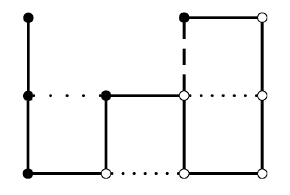
\includegraphics[scale=0.7]{figures/protein_example.png}
	\caption{One possible configuration of  sequence $HHHPHPPPPPH$ in the HP model. There is one $HH$ (represented by a dotted line with wide spaces), one $HP$ (represented by a dashed line) and  two $PP$  (represented by dotted lines) contacts.}
\end{figure}


The total number of topological neighboring positions in the lattice ($z$) is called the lattice coordination number.


For the HP model, an energy function that  measures the interaction between topological  neighbor residues is defined  as  $\epsilon_{HH}=-1$ and $\epsilon_{HP}=\epsilon_{PP}=0$. The HP problem consists of finding the solution that minimizes the total energy. In the linear representation of the sequence, hydrophobic residues are represented with the letter H and polar ones, with P. In the graphical representation, hydrophobic proteins are represented  by black beads and polar proteins, by white beads. Figure~\ref{fig:PROTEXAM} shows the graphical representation of a possible configuration for  the sequence  $HHHPHPPPPPH$ in a 2D space. The energy that the HP model associates with this configuration is $-1$ because there is only one $HH$ contact, arisen between the second and fifth residues.


Among many works related to the Protein Folding Problem, here are some examples of authors and the approaches that have been used to solve it.


%Lin and Su \cite{li2012genetic} proposed an mono objective EA (Evolutionary Algorithm) working with a local search strategy based on pull-moves for the PSP Problem using the simplified model Hydrophobic-Polar 2D (HP-2D). A greedy strategy was employed to avoid inconsistency in the population and to enhance the efficiency of the algorithm. The results show that this approach has better results than the GA within comparable computational times.


%In other work, Lin and Su \cite{lin2011protein} applied a hybrid genetic-based PSO algorithm to HP-3D model with relative representation, optimizing the crossover and mutation operators to improve results in the protein folding process. The algorithm was an improved version of a GA based on a PSO, where the solutions were based to move toward their own best solution.


%Cust\'{o}dio and Dardenne \cite{custodio2014multiple} proposed a Multiple Minima Genetic Algorithm for PSP. The algorithm included a phenotype based crowding mechanism for the maintenance of useful diversity which increases the population's performance and granted the algorithm multiple solutions capabilities instead of.


%The author of \cite{gabriel2012algoritmos} also proposes the use of a multi objective algorithm in tables, similar to the method proposed by \cite{soares2011investigating}, however, using the HP model for the representation and solution evaluation. The author also proposes the use of a second objective that is to measure the distance between hydrophobic amino-acids, allowing the algorithm to distinguish between different solutions with the same energy value.


%Brasil \textit{et al}.\cite{soares2011investigating} proposed a multi objective algorithm in tables and compare its performance with a well-known multi-objective algorithm, the NSGAII \cite{deb2002fast}, optimizing two energy functions, both very important for the folding process: the van der Walls and Electrostatic functions.


Unger and Moult \cite{unger1993genetic} described a genetic algorithm (GA) that uses heuristic-based operators for crossover and mutation for the HP model. The algorithm outperformed many variants of Monte Carlo methods for different instances. Although the good results, the GA was unable to find the optimal solution for the longest instances considered.


The multimeme algorithm (MMA) proposed by \cite{krasnogor2002multimeme} is a GA combined with a set of local search methods. The algorithm for each different instance or individuals in the population, selects the local search method that best fits. Originally used to find solutions for the functional model protein. The algorithm was later improved with fuzzy-logic-based local searches, leading the algorithm to produce improved results in the PSP problem.


In \cite{hsu2003growth}, the author makes use of a Chain growth algorithm, called pruned-enriched Rosenbluth method (PERM), that is based on growing the sequence conformation by adding individuals particles aiming to increase good configurations and eliminating bad ones.


The ant colony optimization (ACO) was also applied to the PSP problem using the HP-2D model in \cite{shmygelska2002ant, shmygelska2003improved}. This approach, utilizes artificial ants  in order to build conformations for a given HP protein sequence. A local search step is also applied to improve the results and maintain the quality of the solutions..

The work of \cite{santana2008protein} describes the use of Estimation of distribution algorithms (EDAs) as an efficient evolutionary algorithm that can learn and exploit the search space regularities in the form of probabilistic dependencies. In the paper was developed new ideas about the application of EDAs to 2D and 3D simplified protein folding problems. What was analyzed is the relation between this proposal and other population-based approaches for the protein folding problem. The obtained results shows tha EDAs can obtain superior results compared with other well-known population based optimization algorithms.


Gabriel \textit{et al}. \cite{gabriel2012algoritmos} proposes the use of a table-based multi objective evolutionary algorithm initially introduced by \cite{delbem2002restabelecimento}, using the HP-3D model for the representation and solution evaluation. The authors also proposes the use of a second objective that aims to measure the distance between hydrophobic amino-acids, allowing the algorithm to distinguish between different solutions with the same energy value.


The present chapter proposes the use of two well-known MOEAs, that have achieved good results when applied to other domains of problems. The main difference between this chapter and the related works \cite{hsu2003growth,krasnogor2002multimeme,shmygelska2002ant,shmygelska2003improved,unger1993genetic, santana2008protein} is the multi-objective formulation. The work of Gabriel \textit{et al}. \cite{gabriel2012algoritmos} inspired the addition of a second objective in the approach that will be presented in this chapter. Although similar, the multi-objective formulation of this chapter is simpler, because it only considers the maximum distance between residues whereas \cite{gabriel2012algoritmos} also considers the average distance between residues. The use of an backtrack initialization strategy and the modification of the mating process are also differences from the previous works. Those modifications were explored in order to improve the results in relation with the standard versions of the MOEAs. Another remarkable difference are the Pareto-based algorithms NSGAII and IBEA that were used in this chapter whilst  Gabriel \textit{et al}. \cite{gabriel2012algoritmos} used a different MOEA proposed by other author.    


%What this work proposes is the use of other well-known algorithms for multi-objective problems, considering the energy minimization and minimization of the size of a conformation as objectives, to analyze and compare its results to the values found in other works considered the state of the art.


\section{Multi-objective Optimization} \label{sec:optimization}


An Evolutionary Algorithm (EA) is an optimization and search technique, highly parallel, inspired by the Darwinian principle of natural selection and genetic reproduction. The nature principles that inspire the EAs are simple. According to the theory of Charles Darwin, the principle of natural selection favors individuals with high fitness, therefore, they have high probability of reproduction. Individuals with more descendants have more chance to perpetuate their genetic code in future generations. The genetic code is what gives the identity of each individual and is represented in the chromosomes. These principles are used in the construction of computational algorithms, that search for better solutions given a specific problem by the evolution of a population of solutions encoded in artificial chromosomes -- data structures used to represent a feasible solution for a given problem in the algorithm execution \cite{pacheco1999algoritmos}.


In general, real world problems have multiple objectives to minimize/maximize and are present in many areas of expertise. To optimize multi objective problems, two or more objectives are considered which are usually conflicting. For these problems it is impossible to find one unique solution. A set of solutions is reached evaluating the Pareto dominance relation \cite{pareto} between the solutions. The main goal is to find the solutions that are non-dominated by any other. A solution dominates other, if and only if, it was better in at least one of the objectives, without being worst in any of the objectives. The set of non-dominated solutions constitutes the Pareto Front. Finding the real Pareto Front is an NP-hard problem \cite{fonseca2005tutorial}, this way, the objective is to find a good approximation to this front.


Multi-Objective Evolutionary Algorithms (MOEAS) are extensions of EAs for multi objective problems that apply the concepts of Pareto dominance to create different strategies to evolve and diversify the solutions. In this work two MOEAs were used: NSGAII \cite{deb2002fast} and IBEA \cite{zitzler2004indicator}.


\subsection{Non-dominated sorting Genetic Algorithm II}


The main characteristic of NSGAII is the application of strong elitism mechanism, that at each generation sets every solution in different fronts according with the non-dominance relation.


Algorithm \ref{alg:nsgaII} receives as inputs a parameter $N$ for the population size and $T$ as maximum number of evaluations. It starts by creating a population of size $N$ called $P_0$. Then $P_0$ is classified according to its calculated fitness and the Non-Dominated-Sort mechanism. The classified $P_0$ is then submitted to a binary tournament operator to select the solutions called parents that will be used to generate the offspring. The parent solutions pass through the crossover and mutation operators generating new solutions called children. At the end of this process the offspring solutions are evaluated and put in a population called $Q_0$.


After this first step, $P_0$ and $Q_0$ are put together and called as an auxiliary population $R$. Through the Non-dominated-sort, $R$ is sorted creating the \textit{fronts}, where solutions from the first \textit{front} are non-dominated by any other solution, and solutions from the second front are dominated only by the solutions of the first front, and so on. For each \textit{front}, its individuals are evaluated by the Crowding-Distance mechanism and those with higher values are stored in the next-generation population called $P_t$ where $t$ is the current evaluation.


After creating and filling $P_t$ with the non-dominated solutions from all \textit{fronts},  the whole $P_t$ has its fitness calculated and then passes through a new process of Binary Tournament, Crossover and Mutation, starting a new cycle in the algorithm.


At the end, after the stop criterion is reached, the algorithm returns a set of non-dominated  solutions.


\begin{algorithm}[htb!]
	\begin{algorithmic}[1]
		\State{$N \gets$ Population Size}
		\State{$T \gets$ Max evaluations}
		\State{$P_0 \gets CreatePopulation(N);$}
		\State{$CalculateFitness(P_0);$}
		\State{$FastNonDominatedSort(P_0);$}
		\State{$Q_0 \gets 0$}
		\While{$Q_0 < N$}
			\State{$Parents \gets BinaryTournament(P_0);$}
			\State{$Offspring \gets CrossoverMutation(Parents);$}
			\State{$Q_0 \gets Offspring$}
		\EndWhile
		\State{$CalculateFitness(Q_0);$}
		\State{$t \gets 0$}
		\While{$t < T$}
			\State{$R_t \gets P_t \cup Q_t;$}
			\State{$Fronts \gets FastNonDominatedSort(R_t);$}
			\State{$P_{t+1} \gets 0$}
			\State{$i \gets 0$}
			\While{$P_{t+1} + Front_i  < N$}
				\State{$CrowdingDistanceAssignment(Front_i);$}
				\State{$P_{t+1} \gets P_{t+1} \cup Front_i$}
				\State{$i \gets i + 1$}
			\EndWhile
			\State{$CrowdingDistanceSort(Front_i);$}
			\State{$P_{t+1} \gets P_{t+1} \cup Front_i[1:(N -P_{t+1})]$}
			
			\State{$Parents \gets BinaryTournament(P_{t+1});$}
			\State{$Q_{t+1} \gets CrossoverMutation(Parents);$}
			\State{$t \gets t +1$}
		\EndWhile
		\State{\Return{$P \gets$ Set of non-dominated solutions.}}
	\end{algorithmic}
	\caption{NSGAII}
	\label{alg:nsgaII}
\end{algorithm}


\subsection{IBEA (Indicator-Based Evolutionary Algorithm)}


%Although single-objective optimization problems may have a unique optimal solution, Multi-objective problems (as a rule) offer a possibly uncountable set of solutions, which when evaluated produce vectors whose components represents trade-offs in decision space \cite{van1998evolutionary}.


In the multi-objective context, optimizing consists in finding a front with good approximation to the \textit{True Pareto Front}. However, there is no general definition about what a "good approximation" of the \textit{True} Pareto front is. Therefore, indicators have been used to evaluate the quality of an approximation front. The \textit{hypervolume} is an example of indicator used for the evaluation and comparison of Pareto front approximation.


In IBEA, quality indicators are used to evaluate the non-dominated set of solutions \cite{figueiredo2013algoritmo}. To use IBEA, it is necessary to define which indicator will be used to associate each ordered pair of solutions to a scalar value. One of the most used indicators is the \textit{hypervolume} due to its capacity of evaluating the convergence and diversity of the search process at the same time  \cite{ishibuchi2008evolutionary}.


\begin{equation} \label{eq:ibea_fitness}
	F(x_i) = \sum_{x_j \in (P-x_i)} {-e^\frac{-I_{Hy}(x_j,x_i)}{k}}
\end{equation}


The IBEA fitness equation is given by Eq. \ref{eq:ibea_fitness} and is used to calculate the contribution of a given solution to the indicator value of a population, where $k$ is a scaling factor depending on $I_{Hy}$, that is the quality indicator, and the underlying problem, being greater than 0, its commonly used with a value of 0.05. The value for $F(x_i)$ corresponds to a quality loss measure of the approximation to the Pareto front if the solution $x_i$ was removed of the population \cite{figueiredo2013algoritmo}, based on the value of $I_{Hy}$, in this case, the \textit{hypervolume}.


Algorithm \ref{alg:ibea} receives as parameters the population size $N$, maximum number of evaluations $T$ and scale factor $k$. It starts by creating a population $P$ of size $N$. Then it repeats the following process until the stop criterion is satisfied: through a Binary Tournament the parents are selected to be used in the Crossover and Mutation operators to generate the offspring and add them to a auxiliary population $\overline P$. After the reproduction step, $\overline P$ is added to $P$. While the size of $P$ exceeds $N$, the worst individual evaluated by the selected indicator is removed from the population, then the population fitness is recalculated. When the algorithm stops, it returns a set of non-dominated solutions found.


\begin{algorithm}[htb!]
	\begin{algorithmic}[1]
	\State{$N \gets$ Population Size}
	\State{$\overline N \gets$ AuxiliaryPopulationSize}
	\State{$T \gets$ Max Evaluations}
	\State{$k \gets$ Scale factor of Fitness}
	
	\State{$P \gets$ CreatePopulation($N$);}
	\State{$\overline P \gets$ CreateEmptyAuxiliaryPopulation($\overline N$);}
	\State{$m \gets 0$}
	\State{CalculateFitness($P$);}
	
	\While{$m \ge T$ or other stop criterion is not reached}
		
		\State{$\overline P \gets$ BinaryTournament($P$);}
		\State{$\overline P \gets$ CrossoverMutation($\overline P$);}
		\State{$P \gets P \cup \overline P$}
		\State{$m \gets m+1$}
		
		\While{Size($P$) $> N$}
			\State{$x^* \gets$ WorstIndividualByFitness();}
			\State{RemoveFromPopulation($x^*$, $P$);}
			\State{CalculateFitness($P$);}
		\EndWhile
	
	\EndWhile
		\State{\Return{$P \gets$ Set of non-dominated solutions}}
	
	\end{algorithmic}
	\caption{IBEA}
	\label{alg:ibea}
\end{algorithm}


\footnotetext[1]{\textit{Hypervolume}: Proposed quality indicators used in the study of \cite{zitzler1998multiobjective}, denoted as the "size of the covered search space". This indicator has two important advantages in relation to others \cite{zitzler2007hypervolume}: 1 - Sensitive to any kind of improvement in the approximation set in relation to other set. 2 - As result of 1, the indicator guarantee that for any approximation set $A$ that has high values of hypervolume, also has all the solutions of the true Pareto front.}


\section{A bi-objective optimization approach to HP protein folding} \label{sec:proposedMethod}


Two multi-objective approaches were designed in this chapter, using the MOEAs (NSGAII and IBEA) described in subsection \ref{sec:optimization}. The relative representation was chosen to represent the chromosomes. Integer vectors are used whereas the genes specifies in which direction, relative to the previous residue, should be placed the next residue. The genes can assume only tree values (0,1,2): 0 indicates that next residue should be placed on right of the previous one, 1 indicates that the next residue should be placed in front of the previous one and 2 indicates that the next residue should be placed on left from the previous. Figure \ref{fig_sim} shows an example of a hypothetical chromosome and the path generated by it in the 2D lattice. The first and second aminoacids were fixed in positions (2,3) and (3,3) respectively. The third aminoacid was placed in (4,3), because the first chromosome gene is 1, and indicates that the aminoacid should be placed in front of the previous. The second chromosome gene is 0, which indicates that the next aminoacid should be placed on the right (4,4) of the previous. The fifth aminoacid was placed in (5,4) because the chromosome gene is 2 and indicates to place the next residue on the right of the previous. The de-codification of the chromosome continues until all aminoacids are placed. Note that chromosome size is always the chain length - 2 because the two first aminoacids are fixed.


\begin{figure}[ht]
	\centering
	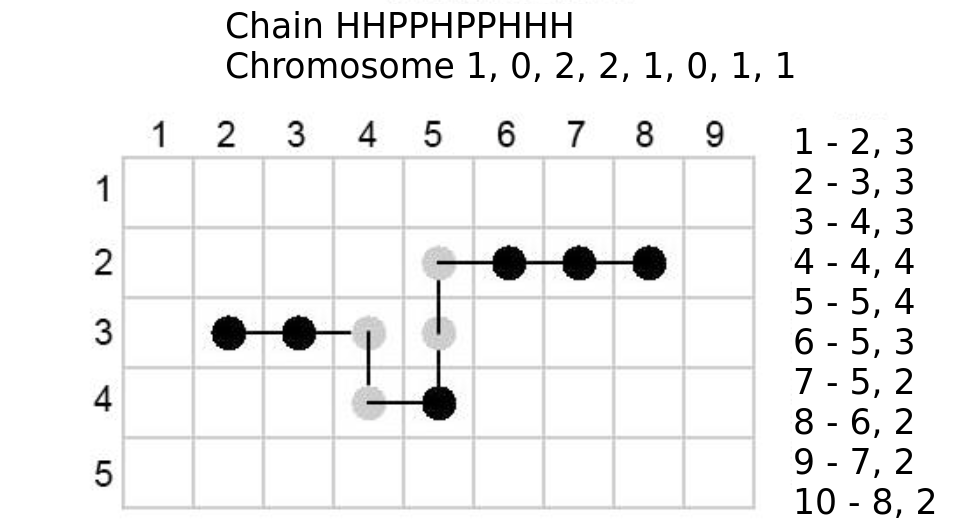
\includegraphics[width=2.5in]{figures/figure3.png}
	\caption{Example of a conformation generated by a chromosome with relative representation.}
	\label{fig_sim}
\end{figure}


The first approach consisted on applying two well-known state of art MOEAs (IBEA and NSGAII) to the PSP using the HP-2D model. The genetic operators used by IBEA and NSGAII algorithms, in this approach, were the single point crossover, and bit flip mutation. This combination of operators presented the best results in preliminary experiments for the PSP problem and the HP-2D model.

In the case of the second approach the IBEA and NSGAII algorithms were modified in order to improve their results when compared with the first approach. The modifications implemented will be described next:

\begin{itemize}
	
	\item \textbf{Pool of operators}: The use of traditional operators usually does not guide the search to prominent regions of the search space of the HP-2D model. In order to improve the MOEAs, a pool of operators was designed based on the literature. For every mating the crossover and mutation operators are selected randomly from the pool of operators and then applied. Also the crossover and mutation operators are always applied this is different from the first approach which uses a probability to apply the operator. The pool of operators will be described next:
	
	\begin{itemize}
		\item Single Point Crossover (1x): A single point on both parent individuals is selected. All data beyond that point in either individual will be swapped between the two parent individuals. Producing two distinct offspring \cite{holland1975adaptation}.
		
		\item Two Point Crossover (2X): Two points are selected on both parent individuals. Everything between the two points is swapped between the parents, building two new distinct individuals \cite{holland1975adaptation}.
		
		\item Multi Point Crossover (MPX): The MPX operator is similar to 2X, but the number of points, $c$, is a function of the sequence length, $n$, given by $c = int(n \times 0.1)$ \cite{custodio2004investigation}. The MPX operator is usually used to promote structural diversity by performing a random shuffle between individuals, although not as thorough as a uniform crossover.
		
		\item Bit Flip Mutation (BFM): The BFM operator selects one random gene from a parent individual and changes it to another value. Resulting in one new individual \cite{holland1975adaptation}.
		
		\item Local Move Mutation (LMM): The LMM operator swaps the directions between two randomly chosen consecutive genes. This operator introduces a corner movement \cite{bazzoli2004memetic}. Figure \ref{fig:operatorLMM} presents an example of application of this operator.
		
		
		
		\begin{figure}[htb!]
			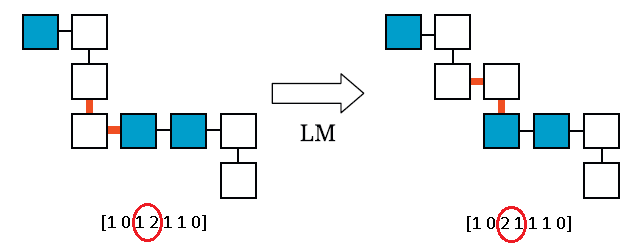
\includegraphics[scale=.4,frame]{figures/operators/LMM.png}
			\label{fig:operatorLMM}
			\centering
			\caption{Example of application of the LMM operator. The genes from the red circle of left figure were swapped resulting in the right figure.} 
		\end{figure}
		
		\item Loop Move Mutation (LOMM): This operator is similar to LMM however this exchanges directions between genes that are five positions apart on the sequence creating a loop movement. Both LMM and LOMM are useful to generate modifications on compact structures \cite{custodio2014multiple}.
		
			\begin{figure}[htb!]
				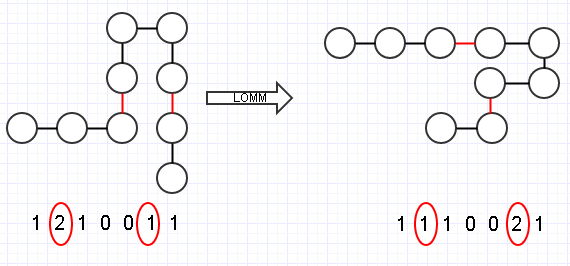
\includegraphics[scale=.4,frame]{figures/operators/LOMM.png}
				\label{fig:operatorLOMM}
				\centering
				\caption{Example of application of the LOMM operator. The genes from the red circle of left figure were swapped resulting in the right figure.} 
			\end{figure}
		
		%Adicionar figura LoMM
		
		\item Segment Mutation (SM): This operator changes a random number of consecutive genes (from two to seven) into new random directions. This operator introduces large conformational changes and has a high probability of creating collisions, in order to avoid too many invalid solutions the repair mechanism is applied on the generated solution \cite{custodio2014multiple}. Figure \ref{fig:operatorSM} demonstrates an application of this operator. 
		
		
			\begin{figure}[htb!]
				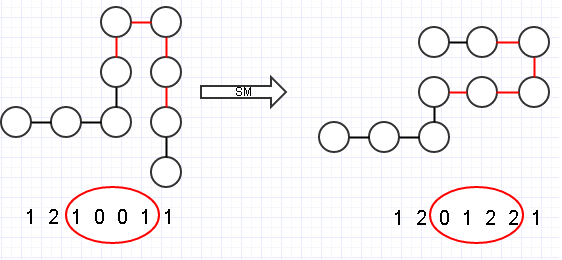
\includegraphics[scale=.4,frame]{figures/operators/SM.png}
				\centering
				\label{fig:operatorSM}
				\caption{Example of application of the SM operator. The genes from the red circle of left figure were swapped by random genes resulting in the right figure.} 
			\end{figure}
		

		
		\item Opposite Mutation (OM): This operator changes a random number of consecutive genes to its inverse position. In the case of the relative representation to the HP-2D model, only left and right directions can be mapped to its inverse. Figure \ref{fig:operatorOM} presents an example of application of this operator.
		
		
		
		\begin{figure}[htb!]
			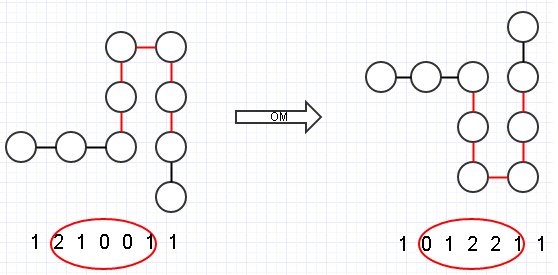
\includegraphics[scale=.4,frame]{figures/operators/OM.png}
			\centering
			\label{fig:operatorOM}
			\caption{Example of application of the OM operator. The genes from the red circle of left figure were swapped by random genes resulting in the right figure.} 
		\end{figure}
		
		
		
	\end{itemize}

	
	\item \textbf{Backtrack Initialization}: Traditionally, the initial population of NSGAII and IBEA are generated randomly. The random based generation of the solutions has a great potential of generating a large number of invalid solutions for the PSP problem within the HP-2D model. Solutions that are not self-avoiding walk (SAW) are said to contain collisions. If the initial population is fully generated randomly the evolutionary algorithms will spend time evaluating invalid solutions. In order to avoid this problem a backtrack strategy should be applied \cite{krasnogor2002multimeme}. In this approach, 20 percent of the initial population was generated using the backtrack initialization.
	
\end{itemize}


For both approaches the following objective functions were used:


\begin{itemize}
	\item \textbf{Energy value}: This is the main objective and consists in the energy of given protein conformation.  The goal is to minimize the energy value and it is calculated as described in section \ref{sec:hpModel}. This objective guides the search progress towards regions that the energies associated to the protein conformations are minimal, thus, achieving protein conformations which are closest to native structure of a protein.
	\item \textbf{Minimize the distance between the two farthest residues}: This is a secondary objective and it was inspired by work presented in \cite{gabriel2012algoritmos}. The motivation for this objective is that more compact conformations tend to have more hydrophobic contacts which means a lesser energy value. The distance between two residues is calculated using the Euclidean distance.
\end{itemize}


The relative representation allows the generation of invalid solutions. A solution is said to be invalid when does not perform a SAW as mentioned before. In other words, an invalid solution is when a given residue collides with another already placed on the lattice. A simple mechanism for repairing these situations was developed, and the code can be seen in the Algorithm \ref{algo:reparacao}.


\begin{algorithm}[h]
	1. The position that the next residue should be placed is obtained 
	2. Verification if the direction selected will cause collision.\\
	3. If a collision is detected, a new direction is used.\\
	4. Repeat the steps 2 and 3, until is possible to place the next residue, or if all directions were tested and cause collisions.\\
	5. If it was possible to place the next residue, the mechanism achieved success, if not, the solution is considered infeasible and it will be penalized in the evaluation process.
	\caption{Mechanism to repair infeasible solutions}
	\label{algo:reparacao}
\end{algorithm}


This mechanism was implemented because in previous experiments it was observed that the number of infeasible solutions was very high. It is necessary to mention that even with the mechanism to repair solutions, there are still infeasible solutions because the mechanism cannot always repair them. Thus, infeasible solutions are penalized by adding the number of collisions to the energy value. This mechanism is used by the evaluation process of both approaches described before (MOEAs without any modifications and the MOEAs supported by the backtracking initialization and the pool of operators).

To evaluate and compare the performance of multi-objective algorithms, quality indicators are commonly used. In this study the hypervolume indicator was used, which considers the volume of the search space dominated by the known Pareto front \cite{zitzler2003performance} of an algorithm. Higher hypervolume value means that the quality of an algorithm is better than one with a lower hypervolume value.


Both approaches were implemented using the open source architecture from  jMetal framework \cite{durillo2011jmetal}.  jMetal is easy to extend, has a well-organized structure and also an active community. 


\section{Experiments} \label{sec:experiments}


This section presents the set of experiments designed to evaluate the performance of the approaches introduced in section \ref{sec:proposedMethod}. The HP sequences used in the experiments are shown in table \ref{tab:instances}. Those instances have been used in previous works such as \cite{bastolla1997testing,shmygelska2002ant,unger1993genetic,cotta2003protein, santana2004protein,shmygelska2003improved,lesh2003complete}. The values presented in table \ref{tab:instances} correspond to the sequence identifier, the size of aminoacid sequence, the best known solutions ($H(x*)$) for the HP-2D model and the sequence itself. It is worthwhile to mention that the sequences used in this chapter were randomly generated. Hence they do not fold to a single conformation, as natural proteins, because they are not products of natural selection \cite{chan2001perspectives}.

\begin{table}[]
	\begin{center}
		\caption{HP instances used in the experiments. The search space of each instance is $2^n$ where $n$ is the size of
			the instance.}
		\label{tab:instances}
		{$\begin{array}{c r r l}
			\text{inst.} & \text{size} &  \multicolumn{1}{ c }{H({\bf{x}}^*)} & \multicolumn{1}{c}{\text{sequence}} \\ \hline
			sq1 &20 &-9 & HPHPPHHPHHPHPHHPPHPH \\
			sq2 &24 &-9 & HHPPHPPHPPHPPHPPHPPHPPHH \\
			sq3 &25 &-8 & PPHPPHHP^4HHP^4HHP^4HH \\
			sq4 &36 &-14 &  P^3HHPPHHP^5H^7PPHHP^4HHPPHPP\\
			sq5 &48 &-23 &  PPHPPHHPPHHP^5H^{10}P^6 \\
			&   &    &  HHPPHHPPHPPH^5 \\
			sq6 &50 &-21 &  HHPHPHPHPH^4PHP^3HP^3HP^4 \\
			&   &    & HP^3HP^3HPH^4{\{PH\}}^4H\\
			sq7 &60 &-36 &  PPH^3PH^8P^3H^{10}PHP^3\\
			&   &    &  H^{12}P^4H^6PHHPHP\\
			sq8 &64 &-42 &   H^{12}PHPH{\{PPHH\}}^2PPH{\{PPHH\}}^2\\
			&   &    &  PPH{\{PPHH\}}^2PPHPHPH^{12}\\
			\hline
			\end{array}$}
	\end{center}
\end{table}

The configuration used for the MOEAs was defined based on the sequence length. For smaller sequences it was used a smaller population size and for larger sequences it was used a larger population size. The same is true in the case of the stop condition (max evaluations). Table \ref{tab:popConfiguration} presents the population size and maximum number of evaluations used for each amino-acid sequence. In the case of the first approach, the probability of crossover/mutation occurrence was fixed, for all sequences, in 0.9 and 0.01 respective. The second approach does not use a probability since the operators are always applied to generate new individuals. The auxiliary population size used by the IBEA algorithm was fixed in 200 for all sequences. For each sequence the algorithms were executed 30 independent times.


\begin{table}[]
	\centering
	\caption{Population size and maximum number of evaluations configurations for each sequence}
	\label{tab:popConfiguration}
	\begin{tabular}{ccccl}
		\hline
		Sequences & Size & \begin{tabular}[c]{@{}c@{}}Population \\ Size\end{tabular} & \begin{tabular}[c]{@{}c@{}}Max \\ Evaluations\end{tabular} & \multicolumn{1}{c}{} \\ \hline
		sq1      & 20   & 100                                                        & 25000                                                      &                      \\ \hline
		sq2      & 24   & 100                                                        & 25000                                                      &                      \\ \hline
		sq3      & 25   & 500                                                        & 250000                                                     &                      \\ \hline
		sq4      & 36   & 500                                                        & 250000                                                     &                      \\ \hline
		sq5      & 48   & 1000                                                       & 2500000                                                    &                      \\ \hline
		sq6      & 50   & 1000                                                       & 2500000                                                    &                      \\ \hline
		sq7      & 60   & 2500                                                       & 2500000                                                    &                      \\ \hline
		sq8      & 64   & 2500                                                       & 2500000                                                    &                      \\ \hline
	\end{tabular}
\end{table}


\subsection{Comparison between the modified/traditional versions of the MOEAs}


As mentioned in the end of section \ref{sec:proposedMethod} the hypervolume indicator was used in order to compare the MOEAs performance. The hypervolume results are presented on table \ref{tab:hypervolumeResults}. The hypervolume average and standard deviation, of 30 independent executions, are presented. The average values highlighted with a bold font are the highest values. 
Looking to table \ref{tab:hypervolumeResults} is possible to notice, except for $sq1$, that for all sequences the M\_IBEA (modified version of the IBEA with backtrack and pool of operators) obtained a higher hypervolume average than the other algorithms. In the case of $sq1$ the IBEA without modifications obtained a higher value compared with the others. It is also possible to see, comparing only the NSGAII versions, that the modified version M\_NSGAII obtained better results, except for $sq1$. In general, the MOEAS with backtrack and pool of operators presented an improvement in relation to the traditional MOEAs. The cells from M\_IBEA that are marked with gray presented statistical difference according to the Kruskal-Wallis test \cite{mckight2010kruskal} between M\_IBEA and all other algorithms (NSGAII, M\_NSGAII and IBEA). 

   

\begin{table}[]
	\centering
	\caption{Results of hypervolume average/standard deviation of the MOEAs}
	\label{tab:hypervolumeResults}
	\begin{tabular}{|c|c|c|c|c|}
		\hline
		\multirow{2}{*}{Instance} & \multicolumn{4}{c|}{\begin{tabular}[c]{@{}c@{}}Hypervolume Average\\ (Std D)\end{tabular}} \\ \cline{2-5} 
		& NSGAII            & M\_NSGAII         & IBEA                     & M\_IBEA                 \\ \hline
		\multirow{2}{*}{sq1}      & 0.742827          & 0.720864          & \textbf{0.789712}        & 0.786571       \\
		& (0.106315)        & (0.131351)        & (0.067660)               & (0.099424)              \\ \hline
		\multirow{2}{*}{sq2}      & 0.680572          & 0.712275          & 0.719960                 & \textbf{0.737086}       \\
		& (0.083445)        & (0.137226)        & (0.080727)               & (0.095299)              \\ \hline
		\multirow{2}{*}{sq3}      & 0.671171          & 0.709898          & 0.716438                 & \textbf{0.738017}       \\
		& (0.129417)        & (0.124201)        & (0.148112)               & (0.155638)              \\ \hline
		\multirow{2}{*}{sq4}      & 0.702280          & 0.740153          & 0.751755                 & \textbf{0.785728}       \\
		& (0689832)         & (0.075271)        & (0.092427)               & (0.055607)              \\ \hline
		\multirow{2}{*}{sq5}      & 0.707654          & 0.758128          & 0.733464                 & \cellcolor[HTML]{C0C0C0}\textbf{0.807637}       \\
		& (0.082611)        & (0.062315)        & (0.128757)               & \cellcolor[HTML]{C0C0C0}(0.039620)              \\ \hline
		\multirow{2}{*}{sq6}      & 0.667771          & 0.774017          & 0.728699                 & \cellcolor[HTML]{C0C0C0}\textbf{0.821177}       \\
		& (0.132218)        & (0.063231)        & (0.080679)               & \cellcolor[HTML]{C0C0C0}(0.048124)              \\ \hline
		\multirow{2}{*}{sq7}      & 0.784483          & 0.792843          & 0.801778                 & \textbf{0.810351}       \\
		& (0.063257)        & (0.033062)        & (0.067111)               & (0.054576)              \\ \hline
		\multirow{2}{*}{sq8}      & 0.677464          & 0.705798          & 0.7450656                & \cellcolor[HTML]{C0C0C0}\textbf{0.811439}       \\
		& (0.041287)        & (0.053048)        & (0.036454)               & \cellcolor[HTML]{C0C0C0}(0.050087)              \\ \hline
	\end{tabular}
\end{table}


\subsection{Comparison between previous single-objective approaches}	


This section presents the comparison of the results obtained by the MOEAs with other approaches from the previous works described on section \ref{sec:hpModel}, and is only concerned with the first objective. (Energy of given conformation), since the other works are single-objective. Table \ref{tab:comparison} presents the best results, in terms of energy, found by the modified MOEAs and also the best results obtained by the previous works.


\begin{table}[]
	\centering
	\caption{Comparison with the previous works}
	\label{tab:comparison}
	\begin{tabular}{ccccccccc}
		\hline
		inst                    & M\_IBEA      & M\_NSGAII    & \begin{tabular}[c]{@{}c@{}}EDA \\ 
			\cite{santana2008protein}
			\end{tabular}           & 
			
			\begin{tabular}[c]{@{}c@{}}GA \\ 
				 \cite{unger1993genetic}
			\end{tabular}   
			
			  & 	\begin{tabular}[c]{@{}c@{}} MMA \\ 
				\cite{krasnogor2002multimeme}  
			  \end{tabular}        
			  &
			  	\begin{tabular}[c]{@{}c@{}}  ACO \\ 
			  		\cite{shmygelska2002ant} 
			  	\end{tabular} 
			  & 
			  	\begin{tabular}[c]{@{}c@{}}  NewACO\\ 
			  		\cite{ shmygelska2003improved} 
			  	\end{tabular}
			  & 
			  \begin{tabular}[c]{@{}c@{}}  PERM\\ 
			  	\cite{hsu2003growth} 
			  	\end{tabular}
			           \\ \hline
		sq1                     & \textbf{-9}  & \textbf{-9}  & \textbf{-9}  & \textbf{-9}  & \textbf{-9}  & \textbf{-9}  & \textbf{-9}  & \textbf{-9}  \\ \hline
		sq2                     & \textbf{-9}  & \textbf{-9}  & \textbf{-9}  & \textbf{-9}  & \textbf{-9}  & \textbf{-9}  & \textbf{-9}  & \textbf{-9}  \\ \hline
		sq3                     & \textbf{-8}  & \textbf{-8}  & \textbf{-8}  & \textbf{-8}  & \textbf{-8}  & \textbf{-8}  & \textbf{-8}  & \textbf{-8}  \\ \hline
		\multicolumn{1}{l}{sq4} & -13          & -13          & \textbf{-14} & \textbf{-14} & \textbf{-14} & \textbf{-14} & \textbf{-14} & \textbf{-14} \\ \hline
		\multicolumn{1}{l}{sq5} & \textbf{-23} & -22          & \textbf{-23} & -22          & -22          & \textbf{-23} & \textbf{-23} & \textbf{-23} \\ \hline
		\multicolumn{1}{l}{sq6} & \textbf{-21} & \textbf{-21} & \textbf{-21} & \textbf{-21} &              & \textbf{-21} & \textbf{-21} & \textbf{-21} \\ \hline
		\multicolumn{1}{l}{sq7} & -35          & -34          & -35          & -34          &              & -34          & \textbf{-36} & \textbf{-36} \\ \hline
		sq8                     & \textbf{-42} & -39          & \textbf{-42} & -37          &              & -32          & \textbf{-42} & -38          \\ \hline
	\end{tabular}
\end{table}


 For the first 3 sequences $sq1$, $sq2$ and $sq3$ the modified MOEAs (M\_NSGAII and M\_IBEA) obtained the same results that the previous works obtained. In the case of $sq4$ both M\_IBEA and M\_NSGAII obtained a value of -13 and all the previous works obtained the optimum value of -14. For sequence $sq5$ four previous works and M\_IBEA have achieved the optimum value -23. However M\_NSGAII and the other previous works obtained a lesser value of -22. In the case of sequence $sq6$ all algorithms obtained the optimum value of -21. For sequence $sq7$ the M\_IBEA obtained -35 as the EDA \cite{santana2008protein}. However the best value found  for $sq7$, -36, were obtained by NewACO \cite{shmygelska2003improved} and PERM \cite{hsu2003growth}. For the last sequence $sq8$ the M\_IBEA obtained the optimum value of -42 which is the same obtained by EDA \cite{santana2008protein} and NewACO \cite{shmygelska2003improved}. All other approaches obtained lesser values for sequence $sq8$.
%TODO pouco discutido


\section{Conclusion and Future works} \label{sec:conclusion}


MOEAs are evolutionary algorithms to address the challenge of optimization of multiple objectives at the same time. They have been showing good results in many areas of science. At this chapter two well known MOEAs were applied in order to address the PSP problem using the HP-2D model. Two multi-objective approaches were presented: the first approach utilizes the standard versions of IBEA and NSGAII algorithms; the second approach consisted on modifying IBEA and NSGAII, adding backtrack initialization and a pool of operators, in order to enhance the results. Given the experiments results it became clear that modified versions of the algorithms were able to explore better the search space than the first approach. 

Also it was possible to check that the multi-objective approach using the NSGAII algorithm, even the modified version (M\_NSGAII), that both of them did not present satisfactory results, comparing with the results achieved by the IBEA variants, in terms of hypervolume. Even that the standard version of IBEA presented better results, when compared with the NSGAII and M\_NSGAII, it not presented good results when compared with the modified version M\_IBEA and with previous single-objective approaches. 

The M\_IBEA was the algorithm that presented better results comparing with NSGAII, M\_NSGAII, IBEA and with the previous single-objective studies. This means that only a multi-objective formulation is not sufficient for achieving good results in terms of energy. Only with the backtrack and the pool of operators the M\_IBEA was able to reach acceptable/competitive results. The multi-objective formulation combined with the backtrack initialization, the pool of operators and the sophisticated mechanism to explore the multi-objective search space of M\_IBEA presented promising results. It is arguably that the M\_IBEA was able to escape from local optima in almost all cases, except for $sq7$, because the capacity of the multi-objective formulation combined with the pool of operators to generated diversity among the population. Also it is worthwhile to mention that the parameters for the algorithms were not tunned and there is a chance of getting better results if a tunning be performed using the M\_IBEA.

The results obtained by the M\_IBEA opens a range of possibilities of exploring further multi-objective formulations to the PSP problem within HP-2D model or even for HP-3D. The findings from this study motivates further approaches using multi-objective designs and the addition of pool of operators in order to enhance the ability of escaping of local optima . In the case of multi-objective formulations it is possible to mention that the design of novel approaches, such as using other metrics to measure the compactness of the proteins conformation or others methods that might consider different characteristics, could improve the ability of MOEAs to reach better results. The open window of opportunities for the pool of goes from the addiction of new operators and better selections methods to 

 Future works include to explore better selection methods to select the operators from the pool operators and also the addition of more operators. It is believed that the pool of operators is the most responsible for the improvement in the exploration of the MOEAs. Therefore more intelligent selection mechanism, which considers the history of the operators application, could improve even more the performance of the MOEAs. The extension of this work to the HP-3D is also planned for the future works. The HP-3D model is more complex than the HP-2D it is possible that the multi-objective approach, presented in this chapter, could suit well. The application of hyper-heuristics is also planned for generation of specialized optimization algorithms for the PSP problem. 

